\section{Results}
\label{sec:results}

\subsection{Moving-MNIST forecast accuracy}
\label{sec:primary}
\label{sec:mm}

\shvar{} improves over \shdet{} in all five replications (Table~\ref{tab:primary}, Figure~\ref{fig:primary}), with a mean paired difference of $\VMMSOneSZeroDiff$ px/frame and 95\% interval $[\VMMSOneSZeroLo,\VMMSOneSZeroHi]$. Its mean Energy Score is \VMMSOneVsSZeroPct\% lower. Against the \emavar{}, \shvar{} scores lower in four of five runs, but the paired difference $\VMMSOneROneDiff$ has interval $[\VMMSOneROneLo,\VMMSOneROneHi]$. The observed means are close, and this interval establishes neither superiority nor equivalence. \shvar{}'s weakest run, replication 1, scores \VMMSOneWeak{} versus \VMMSOneOthersLo--\VMMSOneOthersHi{} for the other four; all five enter the comparison.

\begin{table}[t]
\caption{Moving-MNIST physical-forecast Energy Score ($\downarrow$, px/frame): mean $\pm$ sample SD and range over five paired training replications. Bold marks the lowest observed mean; it does not establish superiority. Appendix Tables~\ref{tab:primary-full} and~\ref{tab:perrep} give both datasets and all 40 runs.}
\label{tab:primary}
\centering
\small
\begin{tabular}{@{}lcc@{}}
\toprule
Model & Energy Score $\downarrow$ (mean $\pm$ SD) & Range \\
\midrule
\emadet{} & 3.254 $\pm$ 0.245 & 2.866--3.537 \\
\emavar{} & 0.777 $\pm$ 0.100 & 0.665--0.881 \\
\shdet{} & 1.625 $\pm$ 0.027 & 1.596--1.659 \\
\shvar{} & \best{0.702 $\pm$ 0.124} & 0.641--0.923 \\
\bottomrule
\end{tabular}

\end{table}

\begin{figure}[t]
\centering
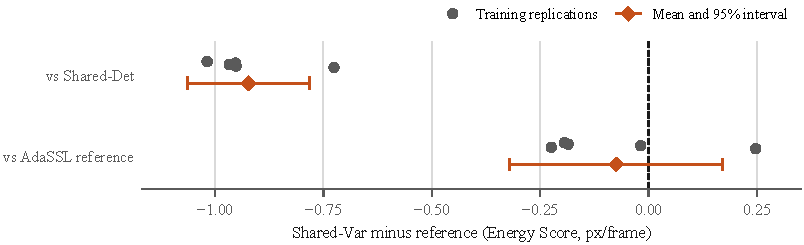
\includegraphics[width=\linewidth]{figures/moving_mnist_paired_comparisons.pdf}
\caption{Moving-MNIST paired differences: \shvar{} minus reference. Circles show the five matched training replications; diamonds and bars show the mean and individual paired-$t$ 95\% interval (4 degrees of freedom). Negative values favour \shvar{}; zero denotes equal scores. Both comparisons use the same scale.}
\label{fig:primary}
\end{figure}

Two references need no learned dynamics: the source-pixel constant-velocity forecast (\VMMPixelCV) and each model's own target-space persistence forecast. \shvar{} beats the pixel forecast in \VMMSOneBeatsPixelCV{} of 5 runs (all but replication 1) and its own persistence in \VMMSOneBeatsPersist{} of 5. The \emavar{} beats the pixel forecast in \VMMROneBeatsPixelCV{} and its own persistence in \VMMROneBeatsPersist{} of 5 runs, and neither deterministic model beats the pixel forecast in any run (Appendix Table~\ref{tab:mmcontrols} and Figure~\ref{fig:physical-full}). These per-run counts are descriptive and do not replace the paired contrast above. The privileged simulator oracle scores \VMMOracle. The \emadet{} scores worst (\VMMRZeroMean), even though decoding its real target embeddings scores \VMMRZeroOracleED.

\subsection{Sampling, readout and representation (secondary)}

\paragraph{Sampling helps within each variational model.} Replacing prior samples with the prior mean worsens the Energy Score in all five runs of each model, by \VMMSOneSamplingGain{} on average for \shvar{} and \VMMROneSamplingGain{} for the \emavar{} (Appendix Figure~\ref{fig:sampling}). At the end of training, the posterior--prior KL on query trajectories averages \VMMSOneKL{} nats for \shvar{} and \VMMROneKL{} for the \emavar{}, so the posterior has not collapsed onto the prior (Appendix Figure~\ref{fig:residual}). The KL is large mainly because the posteriors are much narrower than the prior (mean posterior and prior standard deviations \VMMSOnePostStd{} and \VMMSOnePriorStd{} for \shvar{}); the sampling gain, not the KL, is the evidence that the residual affects forecasts. Empirical 90\% marginal intervals cover \VMMSOneCoverX{}/\VMMSOneCoverY{} of truth draws ($x/y$) for \shvar{} and \VMMROneCoverX{}/\VMMROneCoverY{} for the \emavar{}. These finite-sample coverage estimates do not establish calibration (Appendix Table~\ref{tab:mmresidual} and Figure~\ref{fig:coverage}).

\paragraph{Much of the gap to \shdet{} is present when real futures are decoded.} \shdet{}'s target embeddings encode the new velocity poorly: its readout reaches $R^2=\VMMSZeroReadoutRtwoX/\VMMSZeroReadoutRtwoY$ ($x/y$) on real target clips, against \VMMSOneReadoutRtwoX/\VMMSOneReadoutRtwoY{} for \shvar{}. Decoding real future embeddings already gives an Energy Score of \VMMSZeroOracleED{} for \shdet{} versus \VMMSOneOracleED{} for \shvar{} (Appendix Tables~\ref{tab:mmcontrols} and~\ref{tab:mmrep}). That difference, \VMMOracleGapSZeroSOne{} px/frame, is \VMMOracleGapShare\% of the gap in mean primary scores. Even \shvar{}'s fixed-prior-mean forecasts (\VMMSOneFixedMean) outperform \shdet{}. The primary comparison therefore measures a change in the whole forecasting pipeline: the learned target representation and its readout as well as forecast spread. The design does not separate these effects.

\paragraph{Motion remains decodable, with less digit identity.} Linear digit accuracy on source-clip projector features is \VMMSOneProjDigit{} for \shvar{}, against \VMMSZeroProjDigit{} for \shdet{} and \VMMROneProjDigit{} for the \emavar{}; on backbone features the differences are smaller (\VMMSOneBackDigit{} against \VMMSZeroBackDigit{} and \VMMROneBackDigit). Velocity remains linearly decodable from \shvar{}'s projector ($R^2=\VMMSOneProjVelRtwoX/\VMMSOneProjVelRtwoY$, $x/y$). Relative to \shdet{}, the forecasting gain thus comes with less digit identity at the projector. Appendix~\ref{app:results} gives all probes (Figure~\ref{fig:representation}), readout fidelity (Figure~\ref{fig:fidelity}) and speed-stratified results (Figure~\ref{fig:strata}).

\subsection{MPI3D: no model beats its own persistence forecast on the latent score (secondary)}
\label{sec:mpi3d}

\begin{table}[t]
\caption{MPI3D forecasts over five replications per model ($\downarrow$ lower is better): physical score as mean $\pm$ sample SD, latent score as mean (min--max). Physical scores are in Euclidean grid indices; ``own persistence'' decodes the model's target-space embedding of the source. The latent score is computed in each model's own target space, so it compares each model only with its own persistence (0.5 by construction) and with the true two-outcome distribution (0.25); it does not rank the models. All queries use held-out attribute combinations. Appendix Table~\ref{tab:mpcontrols} gives all controls.}
\label{tab:mpi3d}
\centering
\small
\setlength{\tabcolsep}{3pt}
\begin{tabular}{@{}lccc@{}}
\toprule
 & \multicolumn{2}{c}{Physical ES $\downarrow$ (grid indices)} & Latent ES $\downarrow$ (gap-normalized) \\
\cmidrule(lr){2-3}\cmidrule(l){4-4}
Model & Sampled prior & Own persistence & Sampled prior \\
\midrule
\emadet{} & 4.04$\times$10$^{6}$ $\pm$ 4.03$\times$10$^{6}$ & 3.80 & 2.396 (2.015--2.861) \\
\emavar{} & 4{,}150 $\pm$ 1{,}881 & 3.91 & 1.282 (1.086--1.512) \\
\shdet{} & 7.22 $\pm$ 2.06 & 4.29 & 0.893 (0.777--1.012) \\
\shvar{} & 6.35 $\pm$ 2.23 & 5.92 & 0.750 (0.600--0.913) \\
\midrule
Coordinate persistence (privileged) & \multicolumn{2}{c}{2.00} & -- \\
Two-outcome oracle (privileged) & \multicolumn{2}{c}{1.00} & 0.250 \\
\bottomrule
\end{tabular}

\end{table}

MPI3D tests action-conditioned prediction with two discrete outcomes on held-out attribute combinations (Table~\ref{tab:mpi3d}). On the primary physical score, \shvar{} is lower than \shdet{} in only \VMPSOneSZeroWins{} of 5 replications (mean difference $\VMPSOneSZeroDiff$ grid indices, interval $[\VMPSOneSZeroLo,\VMPSOneSZeroHi]$). Its large difference from the \emavar{}, $\VMPSOneROneDiff$ with interval $[\VMPSOneROneLo,\VMPSOneROneHi]$, does not reflect forecasting skill: the EMA models' predicted features leave the readout's fit support and produce extreme physical scores. Every run scores far above privileged coordinate persistence (\VMPRefCoordPersist). \shvar{}'s readout also transfers less well to the test attributes than the others ($R^2=\VMPSOneReadoutTestRtwo$ on real test targets, against \VMPSZeroReadoutTestRtwo--\VMPRZeroReadoutTestRtwo), so readout error limits its physical scores.

On the decoder-independent latent score, all \VMPLoseToPersistence{} runs score worse than their own persistence control, and \shvar{} averages \VMPSOneLatentES{} against 0.5 for persistence and 0.25 for the true outcome distribution. Only the variational models can beat this control (Section~\ref{sec:evaluation}), and none of their ten runs does (Appendix~\ref{app:mpi3d-results}, Figure~\ref{fig:mpi3d}). In physical units, \shvar{} scores lower than its decoded persistence embedding in \VMPSOneBeatsOwnPhysPersist{} of 5 runs, but readout error dominates both: decoding the real outcome images already scores \VMPSOneOracleED, against \VMPRefOracle{} for the exact distribution, so we base the MPI3D conclusion on the latent score. Because every query uses unseen attribute combinations, the failure may reflect poor compositional generalization as well as poor forecasting; the evaluation cannot separate the two.

\subsection{Fewer stored parameters, dataset-dependent training cost (post hoc)}
\label{sec:cost}

\begin{table}[t]
\caption{\shvar{} relative to the \emavar{} (post hoc, secondary). Negative percentages indicate reductions. FLOPs are analytic matrix-multiplication and convolution counts per training update; stored parameters include the EMA copy, and trainable parameter counts are equal. Equal update budgets give a recipe comparison rather than a cost-matched accuracy comparison. Appendix~\ref{app:cost} gives the absolute values, counter scope and timing measurements.}
\label{tab:costsummary}
\centering
\small
\begin{tabular}{@{}lrr@{}}
\toprule
Dataset & Stored parameters & Training FLOPs / update \\
\midrule
Moving-MNIST & $-37\%$ & $+28\%$ \\
MPI3D & $-42\%$ & $-14\%$ \\
\bottomrule
\end{tabular}

\end{table}

Cost was not a prespecified outcome. We counted FLOPs and parameters and ran the timing benchmark after the main runs; the development wall-clock was recorded from the development runs before main training. Removing the EMA copy reduces stored parameters on both datasets (Table~\ref{tab:costsummary}), but it does not consistently reduce training compute. The difference follows the posterior input. On Moving-MNIST, \shvar{} backpropagates through three encoder passes (source, target and the separate posterior clip), whereas the \emavar{} backpropagates through two and runs its EMA target pass without gradients. \shvar{} therefore uses \VMMCostFlopsVsROne\% more training FLOPs per update. On MPI3D, \shvar{} reuses the target encoding as the posterior input and needs only the two passes of \shdet{}. It uses \VMPCostFlopsVsROne\% fewer FLOPs than the \emavar{} and \VMPCostFlopsVsSZero\% more than \shdet{}. The timing measurements agree in sign (Appendix~\ref{app:cost}, Figure~\ref{fig:cost}). Per-forecast inference compute is the same for the two variational models. The MPI3D saving accompanies forecasts that fail the persistence control.
